\clearpage
\section{Event display}
In this part, we focused on learning how to distinguish different channel by event display and four different variables. All channels have 20 events. 



\subsection{Identification of the particle at the OPAL detector}
To identify the particles, firstly, we divide all particle in charged and uncharged on the basis of visible trajectory in proportional chamber.
The charged hadrons and electrons are separated on the basis of their form and beginning of the shower. The electromagnetic showers caused by an electron have small lateral spread and completely situated with in the electromagnetic calorimeter (ECAL); however, hadronic showers are wider and extended up to the hadronic calorimeter (HCAL). And, muons do not produce any shower.
The neutral particles are identified with the help of different parameters of showers (length, width). The neutral particle decay in to charged particles and follow V tracks.
 

The relevant decay channels are identified as
\begin{enumerate}
\item $ {Z}^0\rightarrow e^+e^- $\\
They create electromagnetic showers through Bremsstrahlung and deposit their energy in the electromagnetic calorimeter. 

\item $ {Z}^0\rightarrow \mu^+\mu^- $\\ 
Muons are heaver than electrons, they don't show showers either Ecal nor Hcal. They penetrate the Hcal and trigger signal in the muon chambers.

\item $ {Z}^0\rightarrow \tau^+\tau-$\\
Tau particles have short life time, so they decay quickly. They can be identified by their decay product. Since they are heavier than electrons and muon and their sum of momentum is less than that electrons and muons for the same energy.

\item $ {Z}^0\rightarrow q\bar{q}$\\
Since quarks cannot exist freely and they form jet of hadrons via strong interaction. Hadronic events have high charge tracks, so they are easy identified.
\end{enumerate}
These events are also visually presented in figure~\ref{fig:eventsDisplay}.

\begin{figure}[H]   
	\begin{minipage}[t]{0.5\textwidth}
		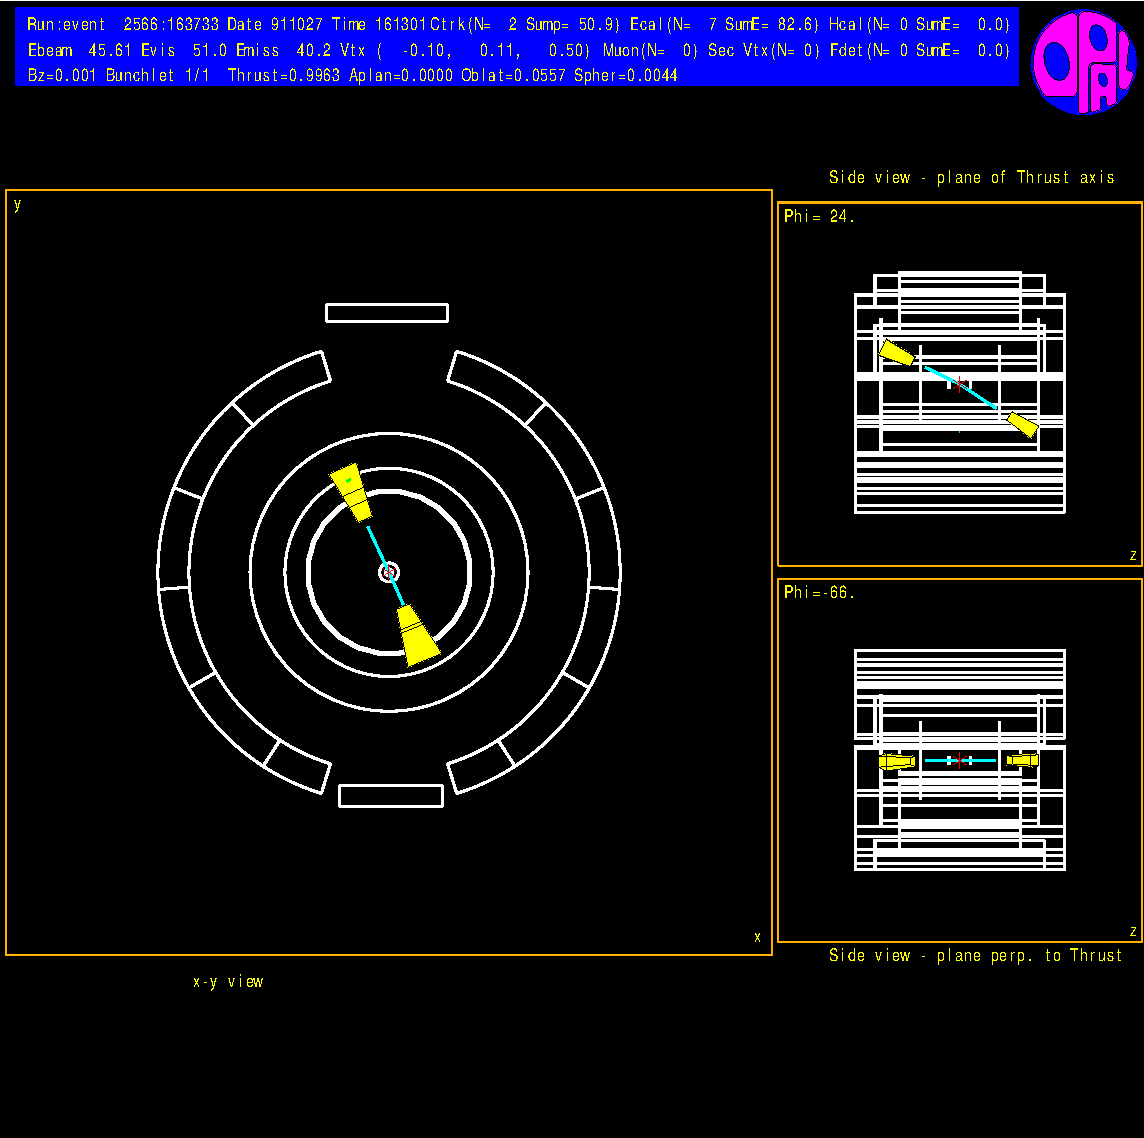
\includegraphics[width=\linewidth]{ee_1.pdf}
		\begin{center}
			{(a) $  {Z}^0\rightarrow e^+e^- $}
		\end{center}
	\end{minipage} \quad
	\begin{minipage}[t]{0.5\textwidth}
		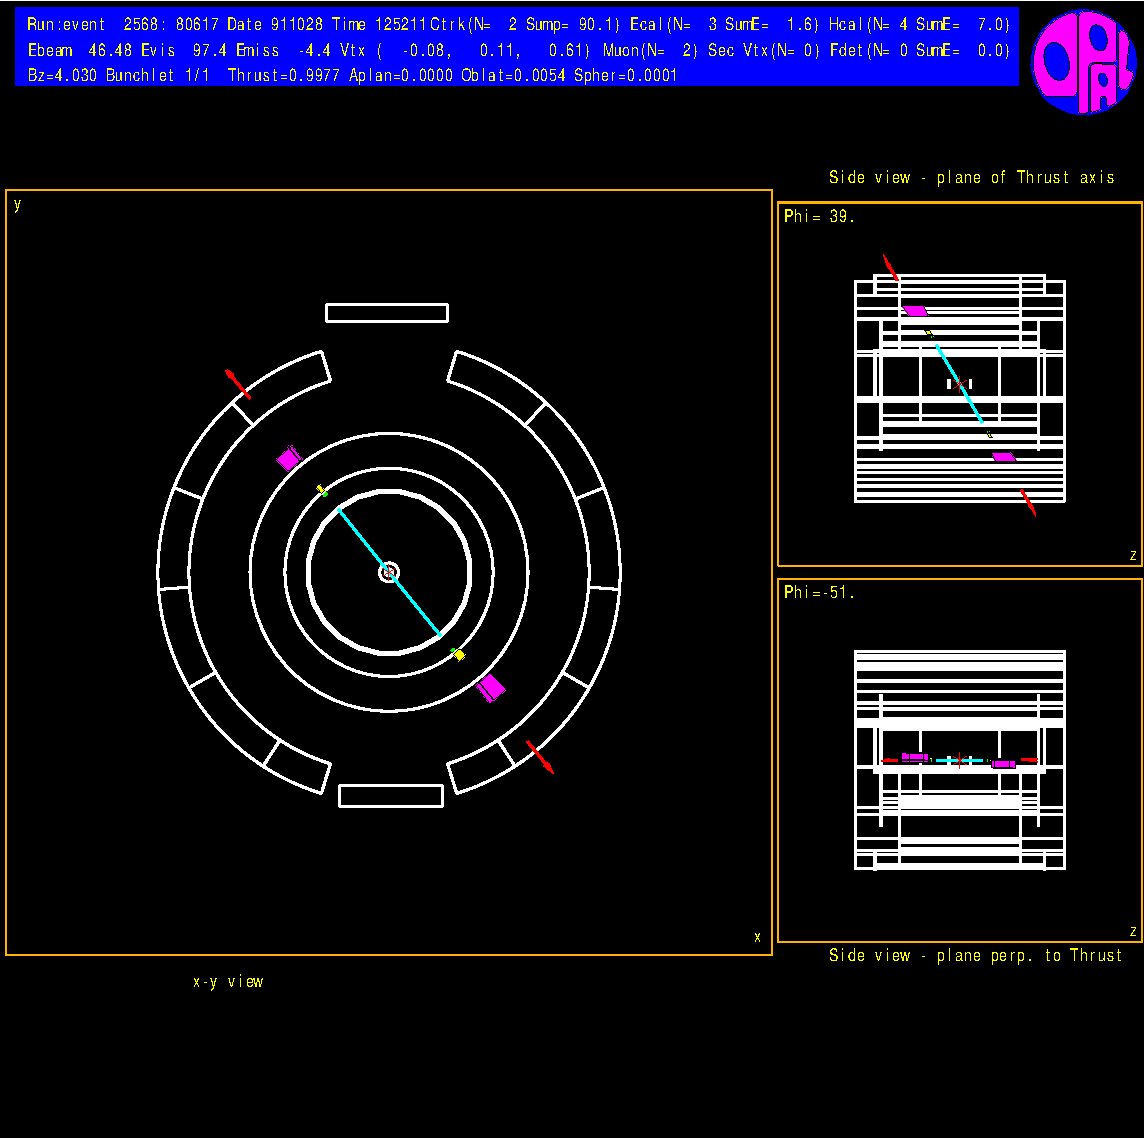
\includegraphics[width=\linewidth]{mm_1.pdf}
		\begin{center}
			{(b) $ {Z}^0\rightarrow \mu^+\mu^- $}
		\end{center}
	\end{minipage}\\
	
	\begin{minipage}[t]{0.5\textwidth}
		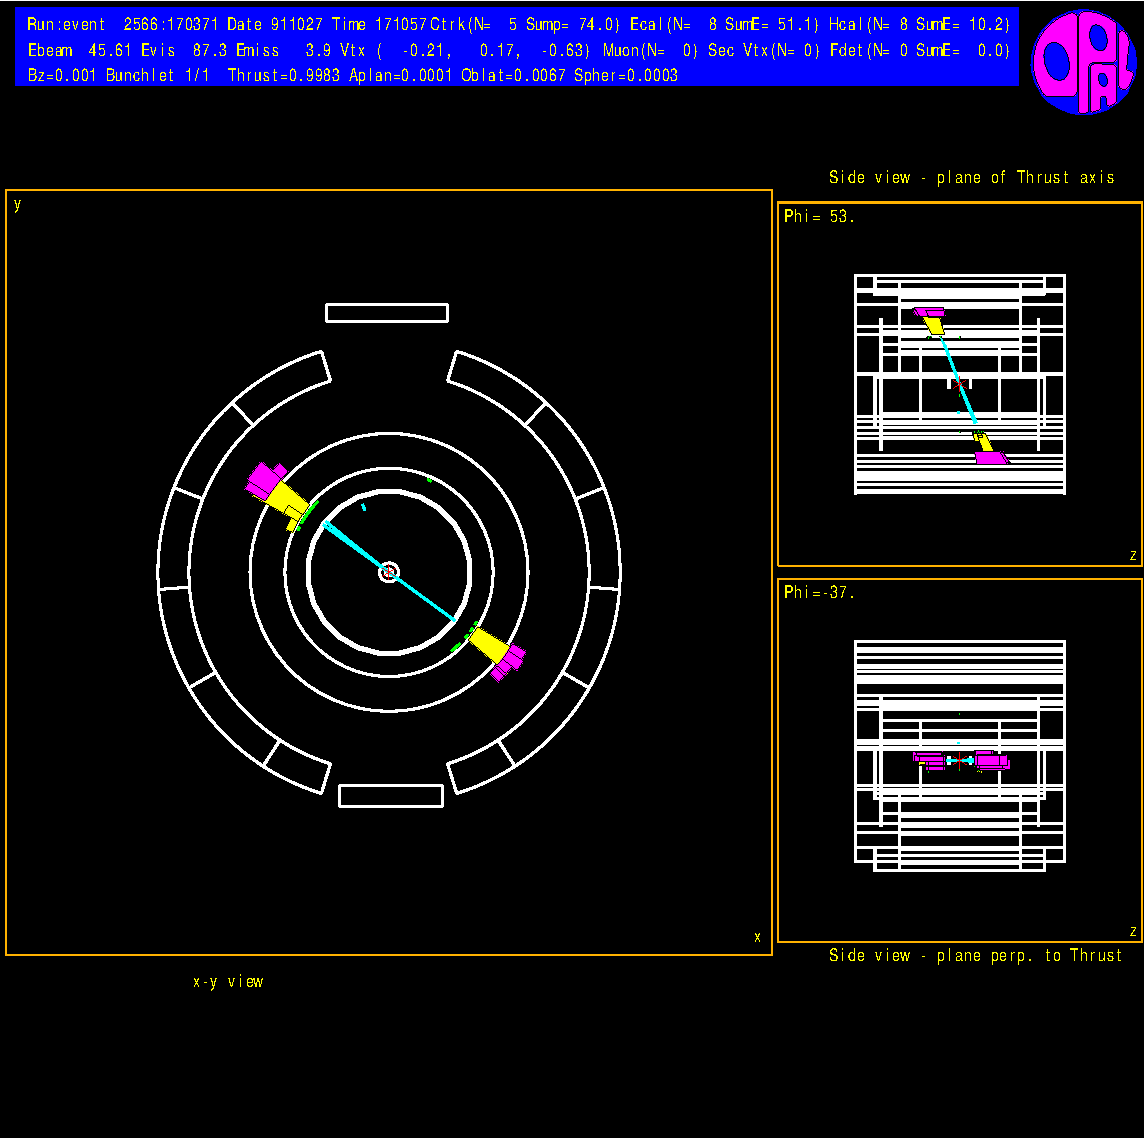
\includegraphics[width=\linewidth]{tt_1.pdf}
		\begin{center}
			{(c) $ {Z}^0\rightarrow \tau^+\tau^- $}
		\end{center}
	\end{minipage} \quad
\begin{minipage}[t]{0.5\textwidth}
		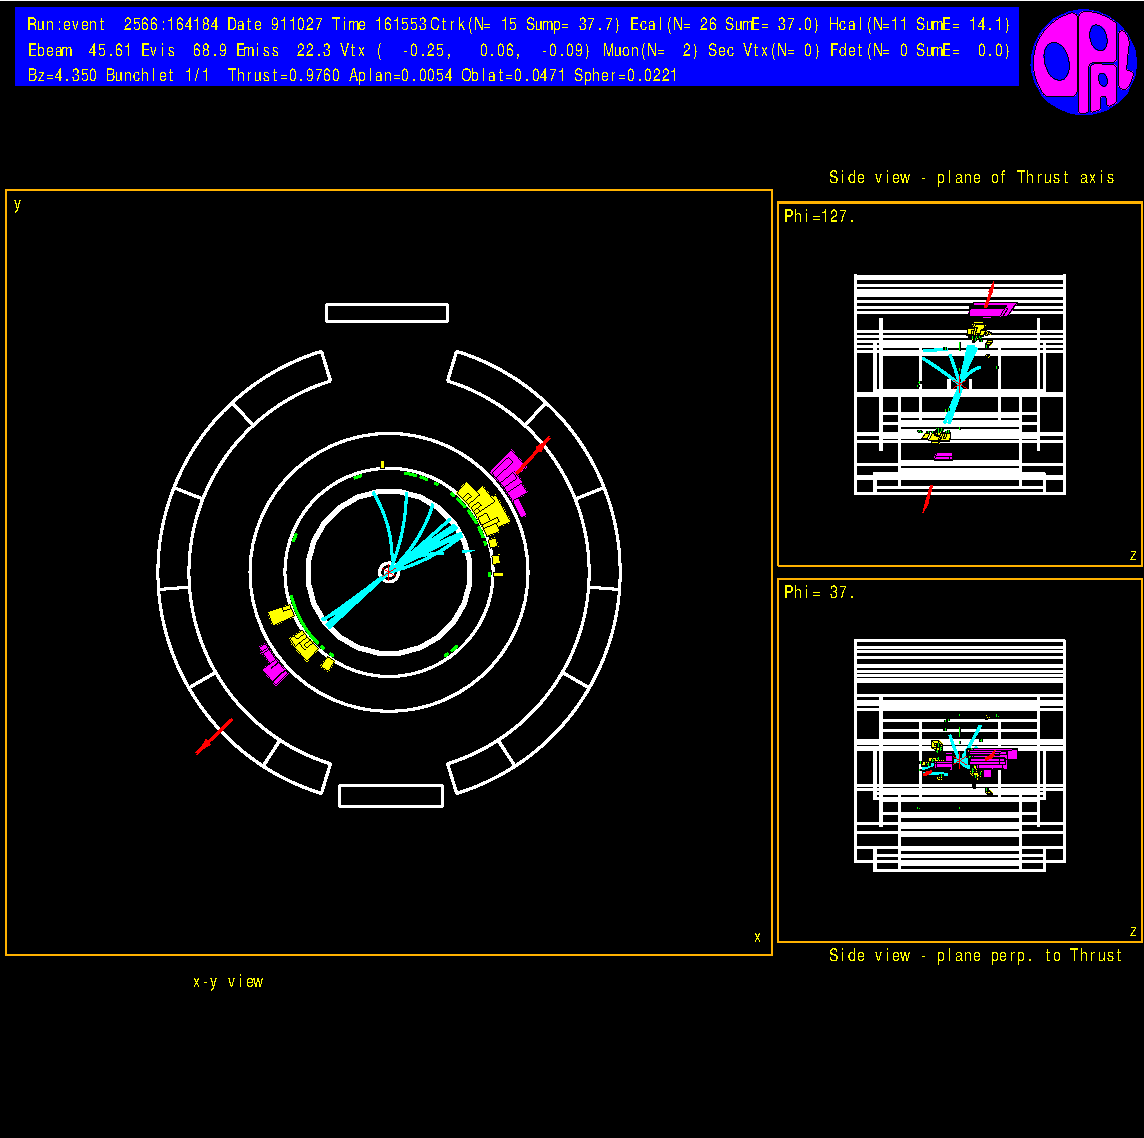
\includegraphics[width=\linewidth]{qq_1.pdf}
		\begin{center}
			{(d) $ {Z}^0\rightarrow q \bar{q}$}
		\end{center}
	\end{minipage}
	\caption{Four different decay modes of $ Z^0 $ boson. Here four important components of OPAL are (from inward to outward): proportional chambers, ECAL, HCAL, and muon chamber.}
\label{fig:eventsDisplay}	
\end{figure}

\subsection{Determination of appropriate cuts for events classification}
In this part we have access to the following variables for each event:
\begin{itemize}
	\item \verb|Ctrk(N)|: Number of charged tracks
	\item \verb|Ctrk(SumP)|: Momentum of all charged tracks
	\item \verb|Ecal(SumE)|: Total energy deposited in the electromagnetic calorimeter
	\item \verb|Hcal(SumE)|: Total energy deposited in the hadronic calorimeter
\end{itemize}

The measured values for each events of channels: $ {Z}^0\rightarrow e^+e^- $, $ {Z}^0\rightarrow \mu^+\mu^- $, $ {Z}^0\rightarrow \tau^+\tau-$,  and $ {Z}^0\rightarrow  $ hadrons of $ Z^0 $ boson are, respectively, listed in tables \ref{tab:ee}, \ref{tab:mm}, \ref{tab:tt}, and \ref{tab:qq} in the appendix.

We plot the histograms for different parameters of different channels and use these to choose the appropriate cuts. Figure~\ref{Fig:histograms_ee} shows the histograms measured in $  {Z}^0\rightarrow e^+e^- $ channel.  
\begin{figure}[H]  
	\begin{subfigure}[t]{0.5\textwidth}
	\begin{center}
		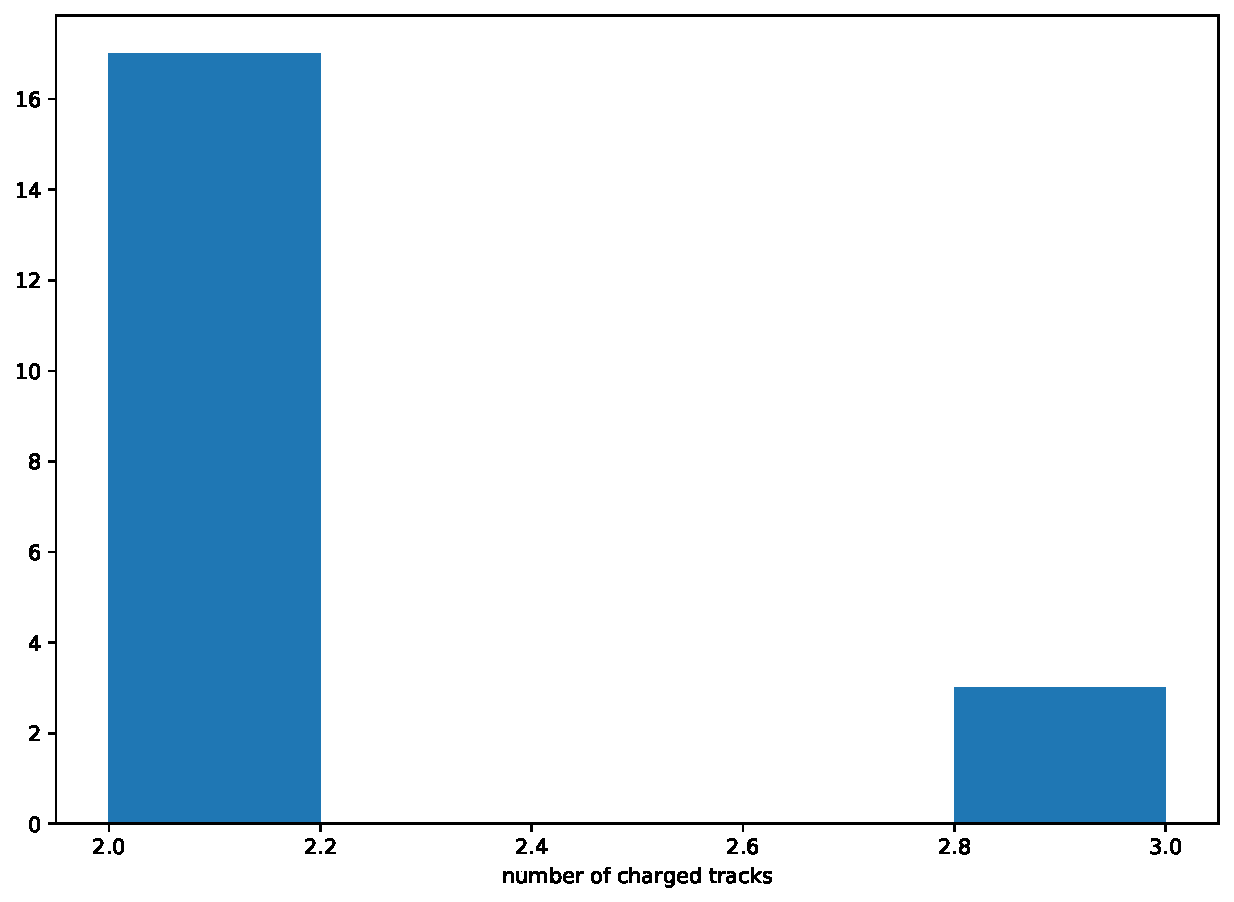
\includegraphics[width=\linewidth]{ee_Ctrk_N.pdf}
	\end{center}
	\caption{Number of charge tracks}
	\label{fig:}
	\end{subfigure}%
	\begin{subfigure}[t]{0.5\textwidth}
	\begin{center}
		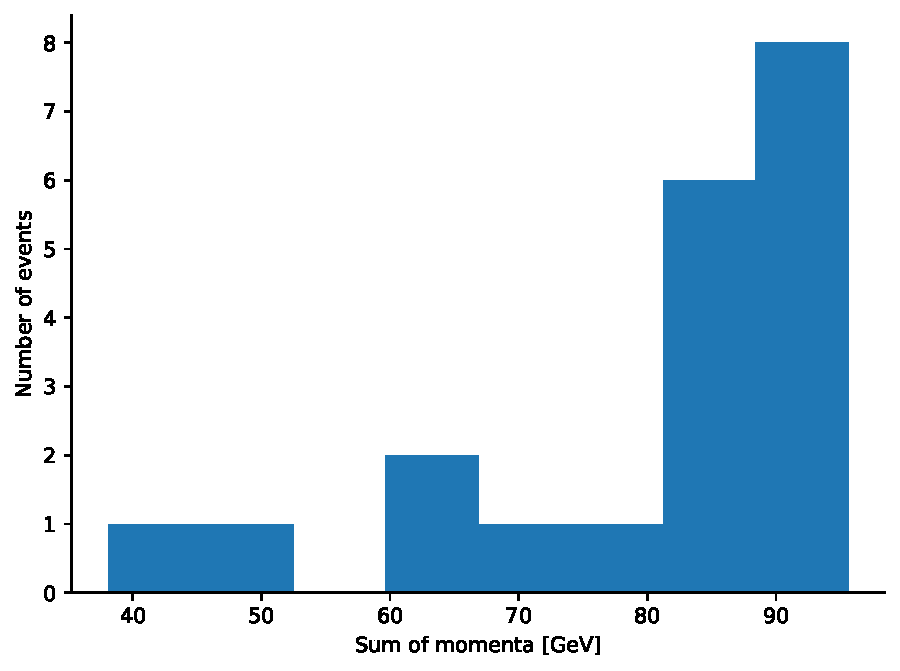
\includegraphics[width=\linewidth]{ee_Ctrl_Sump.pdf}
	\end{center}
	\caption{Total scalar sum of track momenta}
	\label{fig:}
	\end{subfigure}
	
	\begin{subfigure}[t]{0.5\textwidth}
	\begin{center}
		\includegraphics[width=\linewidth]{ee_Ecal.pdf}
	\end{center}
	\caption{Energy deposited in the electromagnetic calorimeter}
	\label{fig:}
	\end{subfigure}%
	\begin{subfigure}[t]{0.5\textwidth}
	\begin{center}
		\includegraphics[width=\linewidth]{ee_Hcal.pdf}
	\end{center}
	\caption{Energy deposited in the hadronic calorimeter}
	\label{fig:}
	\end{subfigure}
	\caption{Histograms of different variables measured in $  {Z}^0\rightarrow e^+e^- $ channel. }
\label{Fig:histograms_ee}	
\end{figure}
From figure~\ref{Fig:histograms_ee}, it is clear that number of charged tracks is pretty low. Sometimes it can be higher than $2$ (ideal case) because of Bremsstrahlung. From this sample, we choose the cut to be $\verb|Ctrk(N)| \leq 3$. As mentioned before, in this decay mode energy deposited in ECAL is significantly large in HCAL. Thus we demand that $\verb|Ecal(SumE)| > 50$ (this will get refined anyway) and $\verb|Hcal(SumE)| < 1$. Sometimes the cuts we set here leave the variable some wiggle room to make sure good identification. There is still pattern in distribution of \verb|Ctrk(SumP)|, but for this part we think aforementioned three cuts are more than enough.

\begin{figure}[H]  
	\begin{subfigure}[t]{0.5\textwidth}
	\begin{center}
		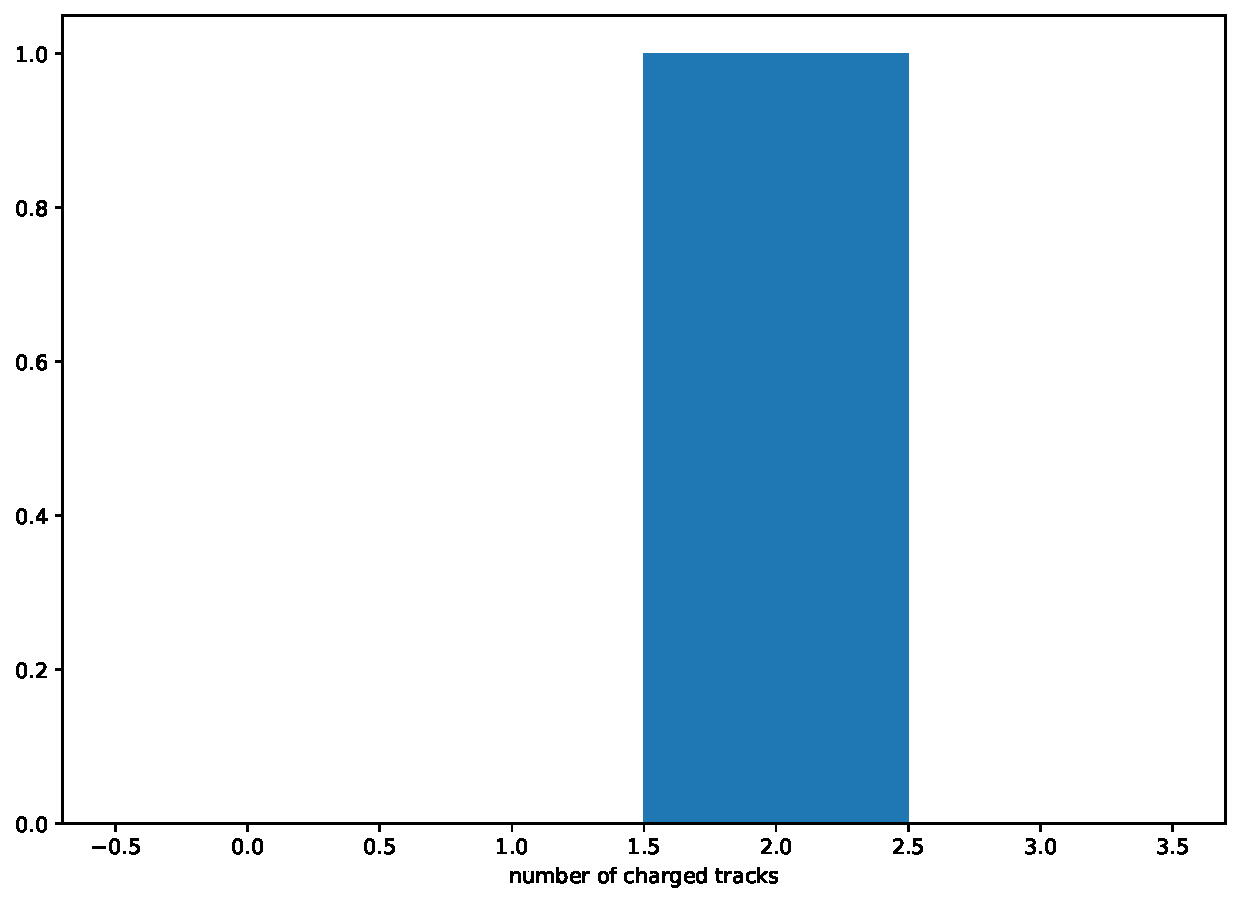
\includegraphics[width=\linewidth]{mm_Ctrk_N.pdf}
	\end{center}
	\caption{Number of charge tracks}
	\label{fig:}
	\end{subfigure}%
	\begin{subfigure}[t]{0.5\textwidth}
	\begin{center}
		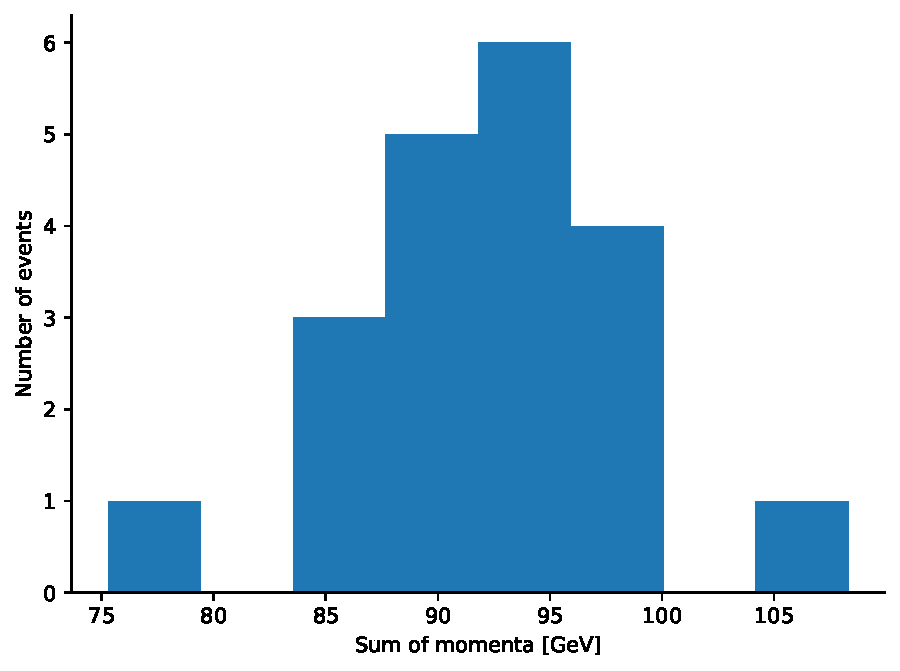
\includegraphics[width=\linewidth]{mm_Ctrl_Sump.pdf}
	\end{center}
	\caption{Total scalar sum of track momenta}
	\label{fig:}
	\end{subfigure}
	
	\begin{subfigure}[t]{0.5\textwidth}
	\begin{center}
		\includegraphics[width=\linewidth]{mm_Ecal.pdf}
	\end{center}
	\caption{Energy deposited in the electromagnetic calorimeter}
	\label{fig:}
	\end{subfigure}%
	\begin{subfigure}[t]{0.5\textwidth}
	\begin{center}
		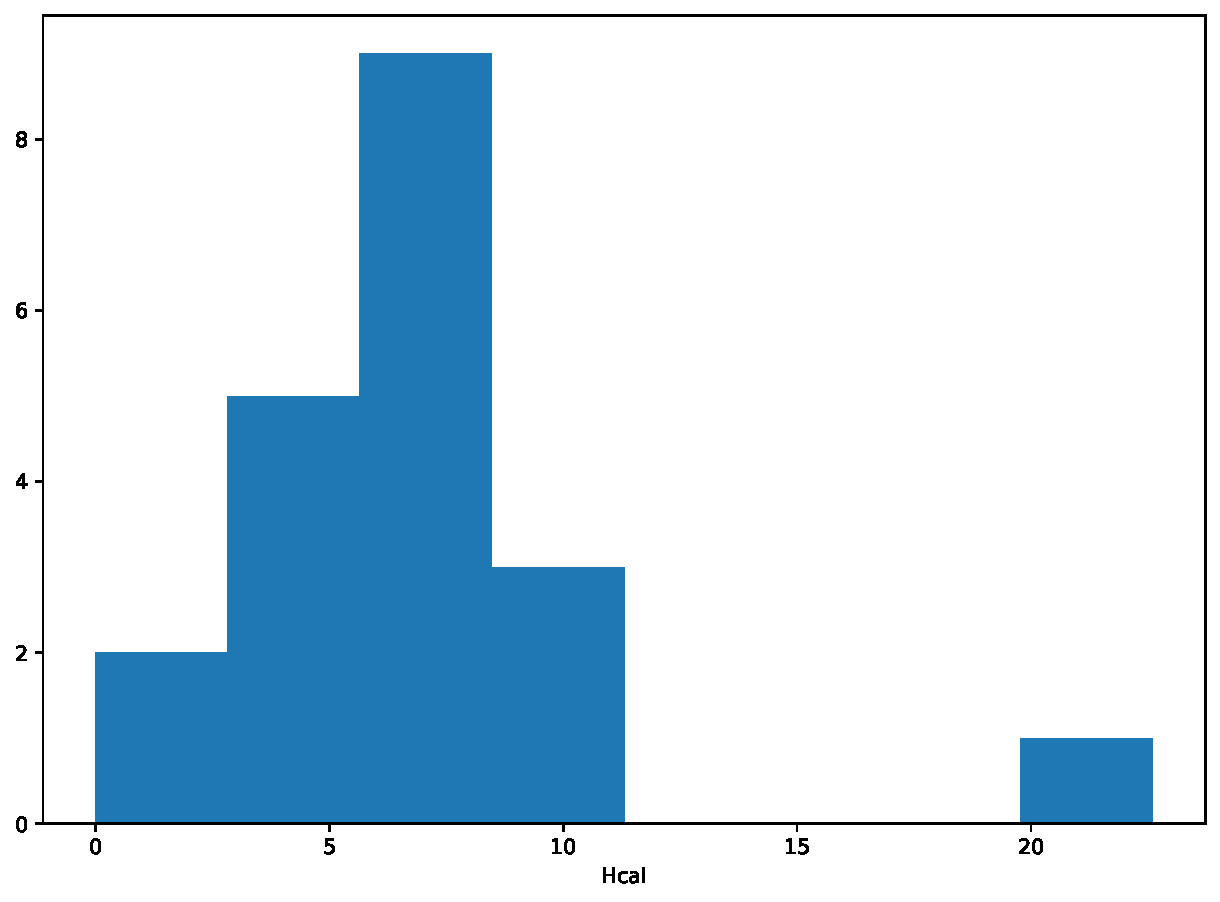
\includegraphics[width=\linewidth]{mm_Hcal.pdf}
	\end{center}
	\caption{Energy deposited in the hadronic calorimeter}
	\label{fig:}
	\end{subfigure}
	\caption{Histograms of different variables measured in $  {Z}^0\rightarrow \mu^+\mu^- $ channel. }
	\label{Fig:histograms_mm}
\end{figure}
In figure~\ref{Fig:histograms_mm}, four histograms are shown and these will be our basis for determining cuts. Similar as $ee$, number of charged track is low, thus a cut $\verb|Ctrk(N)| \leq 3$ is set. Energy of muons mostly goes to muon chamber, thus energies in ECAL and HCAl are quite low. Cuts for these two are set as $\verb|Ecal(SumE)| < 10$ and $\verb|Hcal(SumE)| < 30$. Here a cut in the momenta is set in order to differentiate $\mm$ from $\tta$: $\verb|Ctrk(SumP)| \geq 50$.

\begin{figure}[H]  
	\begin{subfigure}[t]{0.5\textwidth}
	\begin{center}
		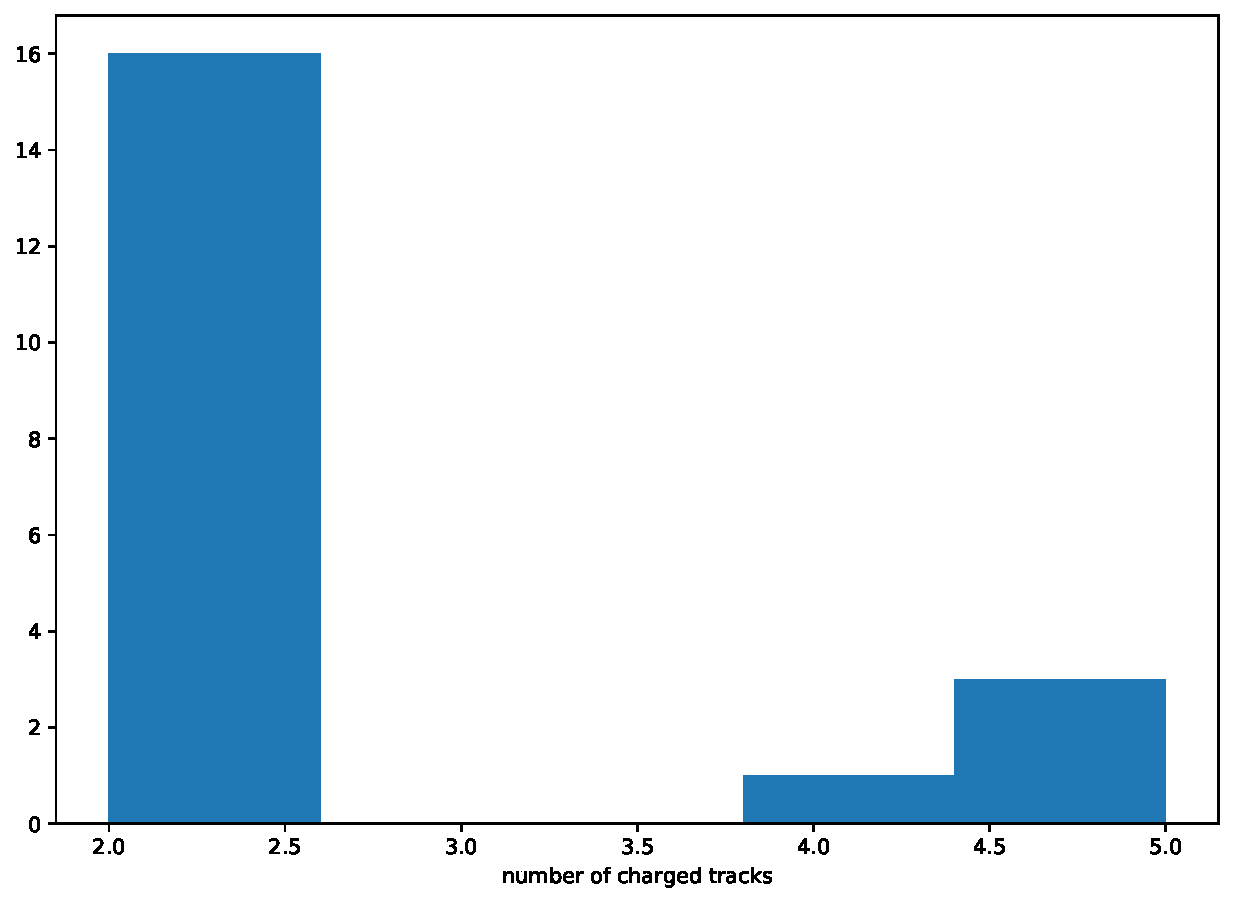
\includegraphics[width=\linewidth]{tt_Ctrk_N.pdf}
	\end{center}
	\caption{Number of charge tracks}
	\label{fig:}
	\end{subfigure}%
	\begin{subfigure}[t]{0.5\textwidth}
	\begin{center}
		\includegraphics[width=\linewidth]{tt_Ctrl_Sump.pdf}
	\end{center}
	\caption{Total scalar sum of track momenta}
	\label{fig:}
	\end{subfigure}
	
	\begin{subfigure}[t]{0.5\textwidth}
	\begin{center}
		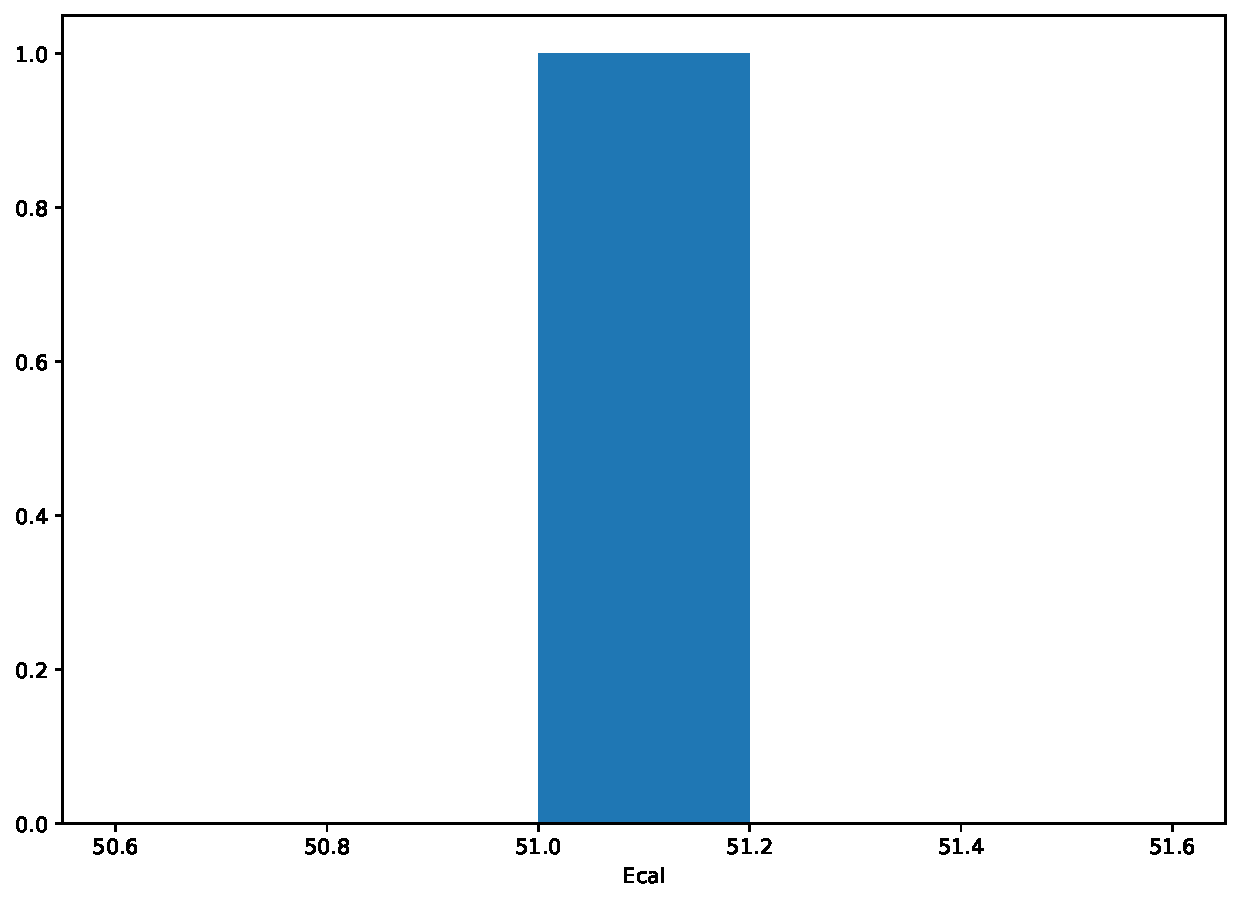
\includegraphics[width=\linewidth]{tt_Ecal.pdf}
	\end{center}
	\caption{Energy deposited in the electromagnetic calorimeter}
	\label{fig:}
	\end{subfigure}%
	\begin{subfigure}[t]{0.5\textwidth}
	\begin{center}
		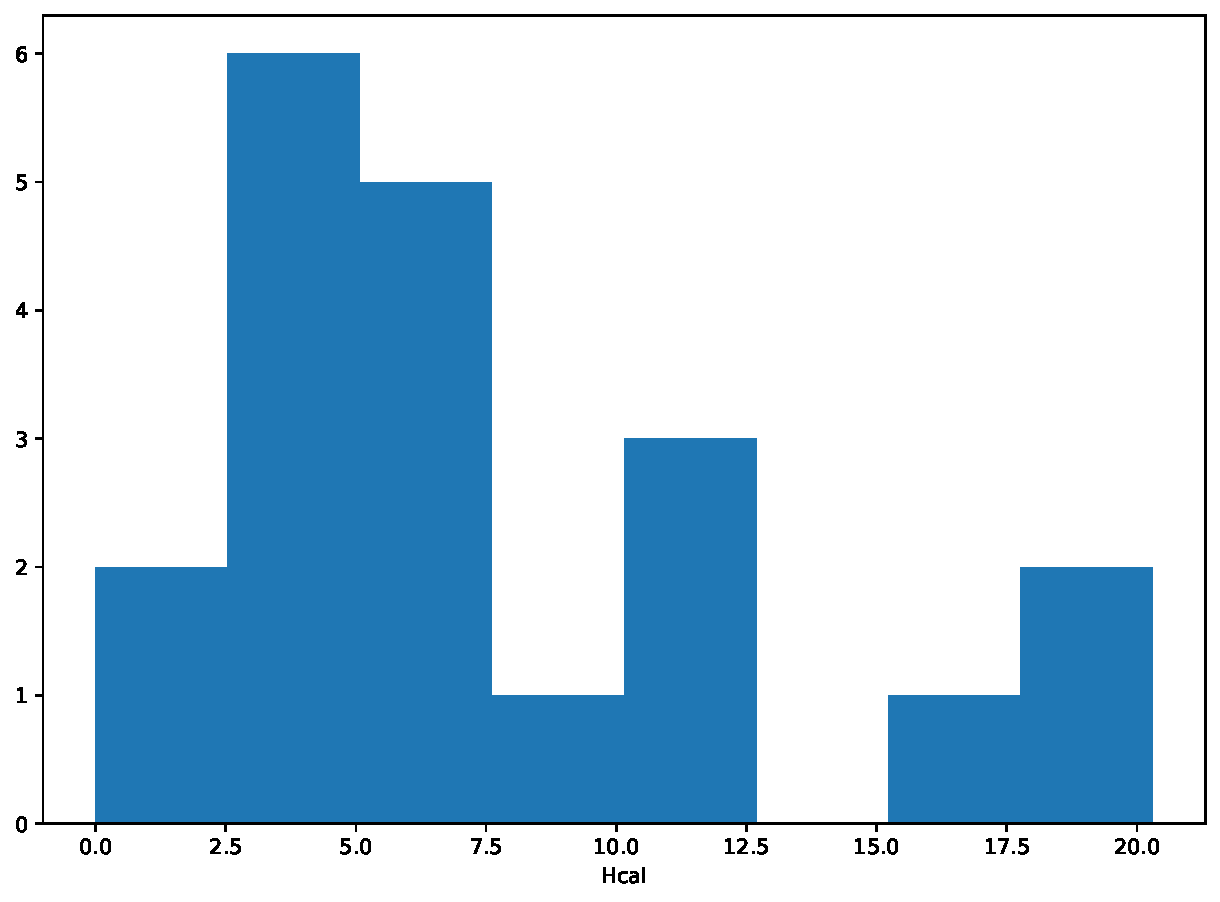
\includegraphics[width=\linewidth]{tt_Hcal.pdf}
	\end{center}
	\caption{Energy deposited in the hadronic calorimeter}
	\label{fig:}
	\end{subfigure}
	\caption{Histograms of different variables measured in $  {Z}^0\rightarrow \tau^+\tau^- $ channel. }
	\label{Fig:histograms_tt}
\end{figure}
Figure~\ref{Fig:histograms_tt} shows distributions of variables in $\tta$ channel. Again the number of charged track is low. But since $\tau$ can decay into charged hadrons also, we set the cut at $\verb|Ctrk(N)| \leq 7$. Two constraints on energy in ECAL and HCAL are set to $\verb|Ecal(SumE)| < 60$ and $\verb|Hcal(SumE)| < 30$. Compared to $\mm$ channel, $\tta$ has relatively low sum of momenta, thus $\verb|Ctrk(SumP)| < 75$. 

\begin{figure}[H]  
	\begin{subfigure}[t]{0.5\textwidth}
	\begin{center}
		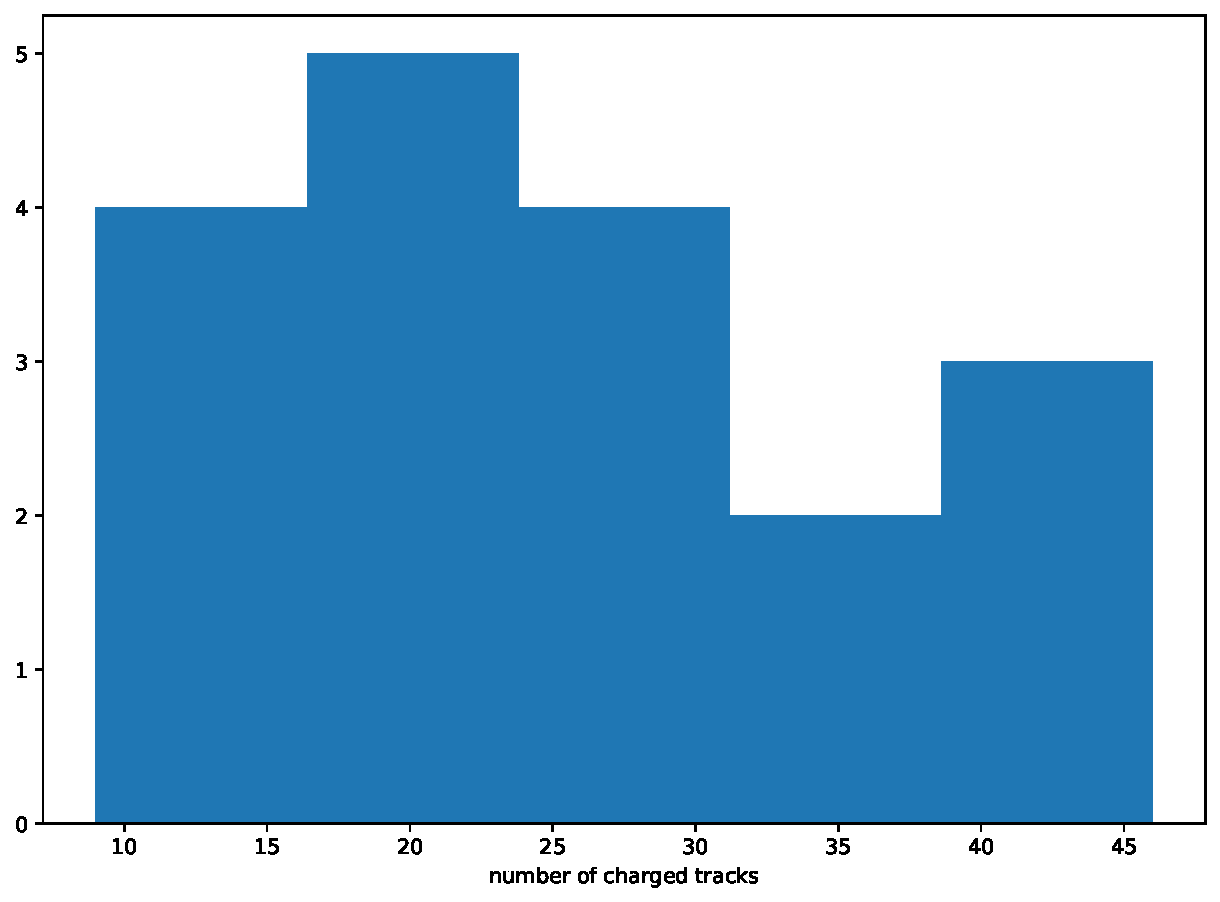
\includegraphics[width=\linewidth]{qq_Ctrk_N.pdf}
	\end{center}
	\caption{Number of charge tracks}
	\label{fig:}
	\end{subfigure}%
	\begin{subfigure}[t]{0.5\textwidth}
	\begin{center}
		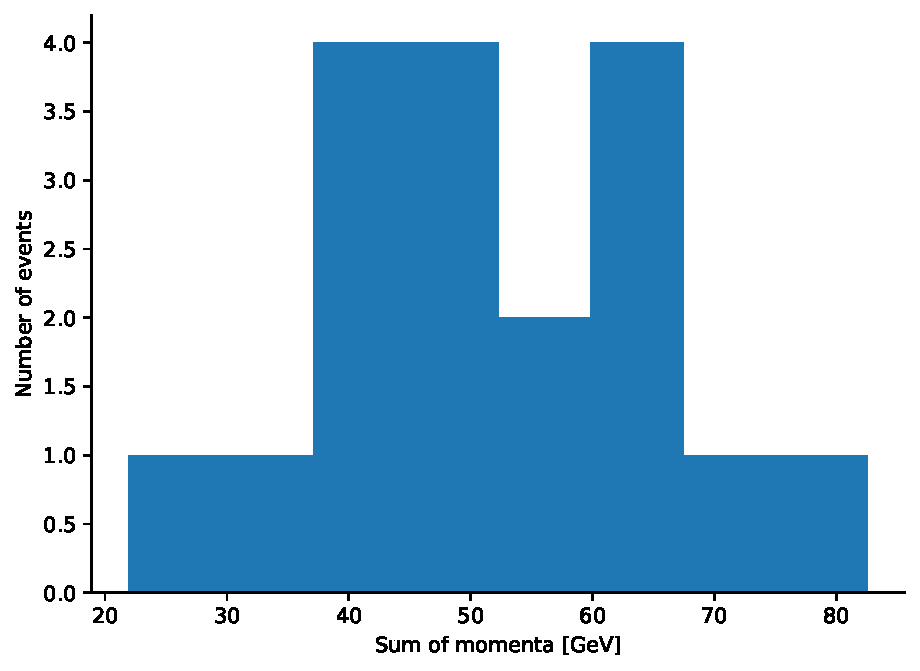
\includegraphics[width=\linewidth]{qq_Ctrl_Sump.pdf}
	\end{center}
	\caption{Total scalar sum of track momenta}
	\label{fig:}
	\end{subfigure}
	
	\begin{subfigure}[t]{0.5\textwidth}
	\begin{center}
		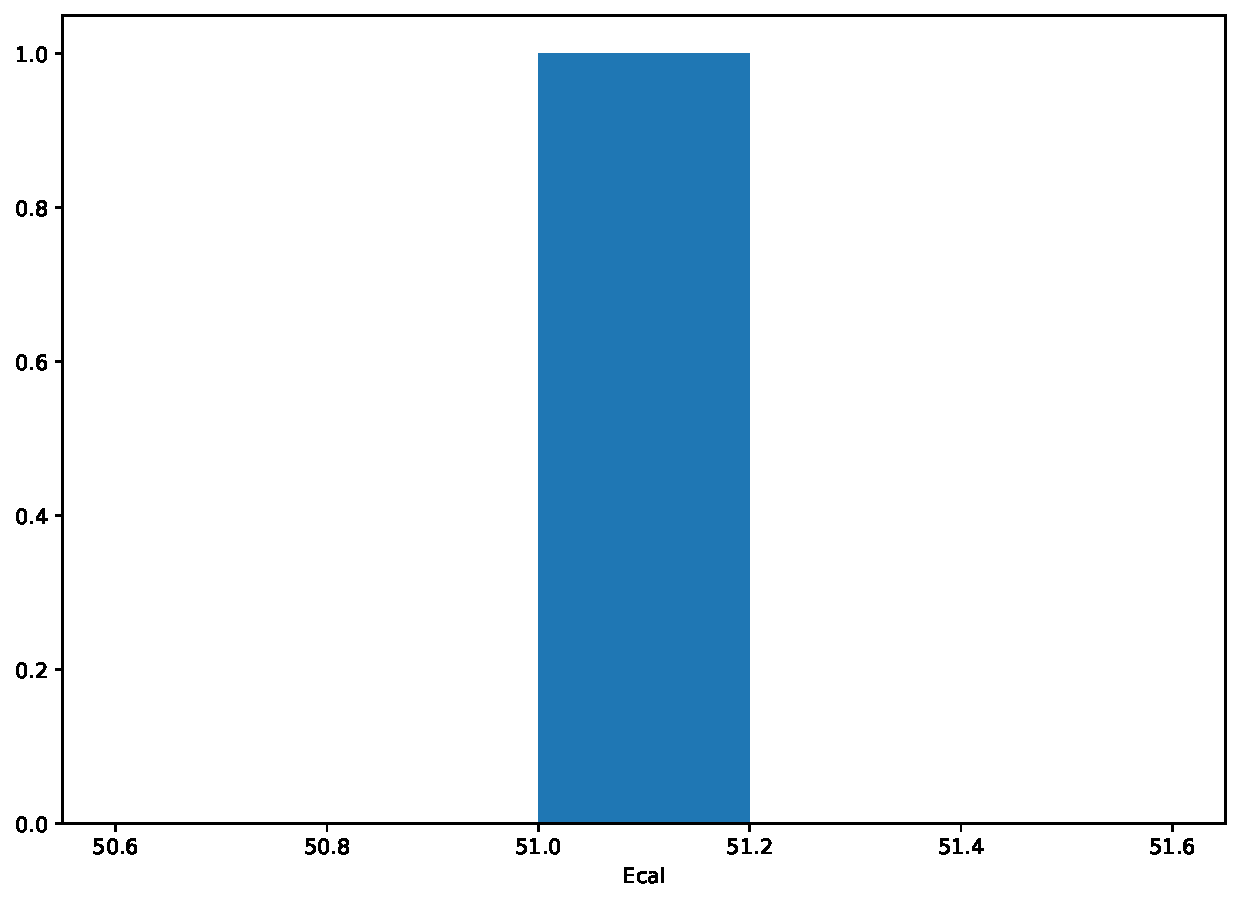
\includegraphics[width=\linewidth]{qq_Ecal.pdf}
	\end{center}
	\caption{Energy deposited in the electromagnetic calorimeter}
	\label{fig:}
	\end{subfigure}%
	\begin{subfigure}[t]{0.5\textwidth}
	\begin{center}
		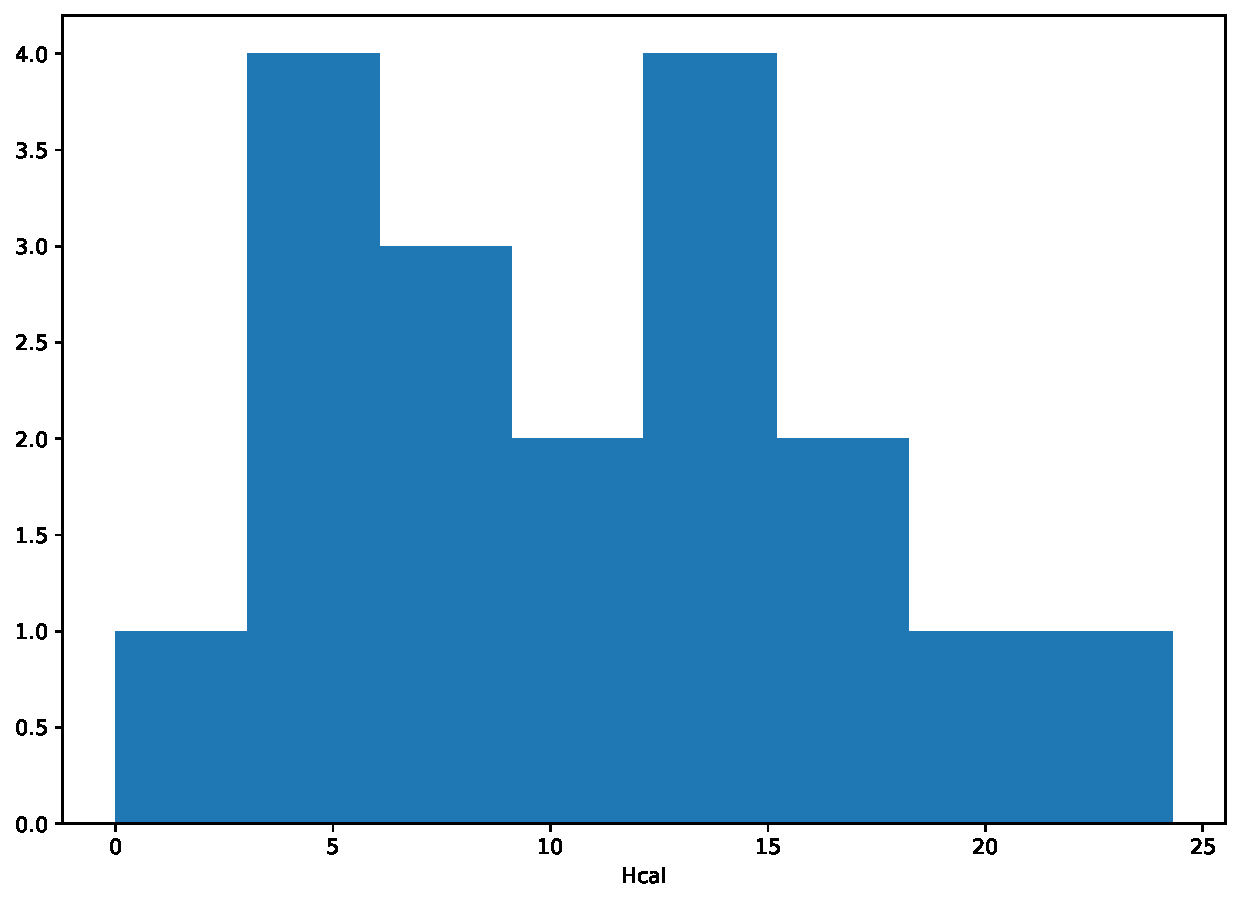
\includegraphics[width=\linewidth]{qq_Hcal.pdf}
	\end{center}
	\caption{Energy deposited in the hadronic calorimeter}
	\label{fig:}
	\end{subfigure}
	\caption{Histograms of different variables measured in $  {Z}^0\rightarrow qq $ channel. }
	\label{Fig:histograms_qq}
\end{figure}
Finally the histograms of $qq$ channel is shown in figure~\ref{Fig:histograms_qq}. Very obvious, number of charged track is large, thus $\verb|Ctrk(N)| \geq 7$ is set. In principle it is enough, but we introduce another cut: $\verb|Ecal(SumE)| > 30$, since we know that hadrons do deposit some energy into ECAL.

We understand there are some overlaps of cuts of $\mm$ and $\tta$, but this ambiguity never shows up in the test data and cuts need to improved later anyway. There are also some events potentially cannot belong to any of these categories. It is fine, as long as the corresponding cut efficiency is good. Our cuts all together are listed in table \ref{Tab:cuts}.
\begin{table}[H]
	\centering
	\begin{tabular}{ccc ccc}
		\toprule
		channel & \verb|Ctrk(N)| & \verb|Ctrk(Sump)| & \verb|Ecal(SumE)| & \verb|Hcal(SumE)| \\
		\midrule
		$ee$ & $ \le 3$  &   &    $ > 50$  & $<1$	\\
		$\mm$ &  $ \le 3$  &  $ \ge 50$  &    $< 10$  & $< 30$	\\
		$\tta$ &  $ \le 7$  & $< 75$  & $ < 60$    & $< 30$	\\
		$qq$ &  $ \ge 7$ &   &  $> 30$    &	\\
		\bottomrule
	\end{tabular}
	\caption{Measured Cuts for different variables of different channels. Unit for energy and momenta is as always \si{\giga\eV}.}
	\label{Tab:cuts}
\end{table}
\subsection{Event classification for test sample}

	
To classify events from the sample \verb|test1| we used the cuts from table \ref{Tab:cuts}. To do so, firstly, we checked the \verb|CtrkN| to pick out hadrons particle from others, also we verified \verb|Ecal| number. Secondly, we check the values of \verb|Ecal| and \verb|Hcal| to verified electrons. Finally, we checked the value of \verb|CtrkSump| as well as \verb|Ecal| and \verb|Hcal| to conform the muons or tauons. The measured valued for each variables and the decay channel classification result are given table \ref{tab:test1}.
\begin{table*}[htbp]
	\centering
	
	\begin{tabular}{ccc ccc}
		\toprule
		Event & Ctrk(N) & Ctrk(Sump) & Ecal(SumE) & Hcal(SumE) & Comment \\
		\midrule

1& 19& 39.5&44.3&15.6 & $ \text{z}^0\rightarrow q\bar{q}$\\
2& 36& 42.8&57.1&12.5& $ \text{z}^0\rightarrow q \bar{q}$\\
3& 2& 95.7& 93.4&0.0& $ \text{z}^0\rightarrow e^+e^- $\\
4& 2& 90.8&1.4&4.1& $ \text{z}^0\rightarrow \mu^+\mu^- $\\
5& 4& 36.5&35.8&10.8& $ \text{z}^0\rightarrow \tau^+\tau-$\\
6& 2& 97.0&2.2&8.9& $ \text{z}^0\rightarrow \mu^+\mu^- $\\
7& 68& 42.9&48.5&6.2& $ \text{z}^0\rightarrow q\bar{q}$\\
8& 5& 35.0&40.8&3,3& $ \text{z}^0\rightarrow \tau^+\tau-$\\
9& 21& 75.8&45.8&21.0&$ \text{z}^0\rightarrow q \bar{q}$\\
10& 2& 95.2&1.3&7.9& $ \text{z}^0\rightarrow e^+e^- $\\
11& 2& 22.7&34.4&0.0& $ \text{z}^0\rightarrow \tau^+\tau-$\\
12& 4& 44.3&37.8&2.6& $ \text{z}^0\rightarrow \tau^+\tau-$\\
13& 21& 53.1&36.2&22.9& $ \text{z}^0\rightarrow q\bar{q}$\\
14& 2& 89.5&92.0&0.0& $ \text{z}^0\rightarrow e^+e^- $\\
15& 2& 89.1&89.7&0.0& $ \text{z}^0\rightarrow e^+e^- $\\
16& 2& 4.1&4.4&0.0& $ \text{z}^0\rightarrow \tau^+\tau-$\\
17& 2& 87.8&1.4&4.3& $ \text{z}^0\rightarrow \mu^+\mu^- $\\
18& 2& 75.3&90.0&0.0& $ \text{z}^0\rightarrow e^+e^- $\\
19& 2& 93.7&1.6&6.8& $ \text{z}^0\rightarrow \mu^+\mu^- $\\
20& 2& 67.1&93.6&0.0& $ \text{z}^0\rightarrow e^+e^- $\\
\bottomrule
\end{tabular}
\caption{Measured parameter for $ \text{z}^0\rightarrow $ hadrons channel}
\label{tab:test1}
\end{table*}

